\chapter{Sana System}
Sana System is belived to be an Iranian malware targeting Iranian cellphones. The virus logs the user phone number and sends it to a remote server. In addition the virus also reads every incoming SMS messages and sends them to the aforementioned server, this could be used to steal sensitive information like 2FA codes. After doing some online research we discovered an article were it is mentioned that a similar virus with the same app name is installed from a fake minister of justice site where the user also insert his bank account information under the pretext of showing juridical documents and, after infecting the user phone, sends malicious links to other phone contacts to spread the virus. We are certain that the viruses are different since the one we analyzed does not have any permission to access contacts info and write messages, however, due to the stunning similarity in presentation and SMS handling, we decided to point out this thing. This could be indicate them being part of the same phishing campaign originating from the same group.

\section{VirusTotal}
We started by feeding the APK to the VirusTotal tool:
\begin{figure}[h!]
\centering
    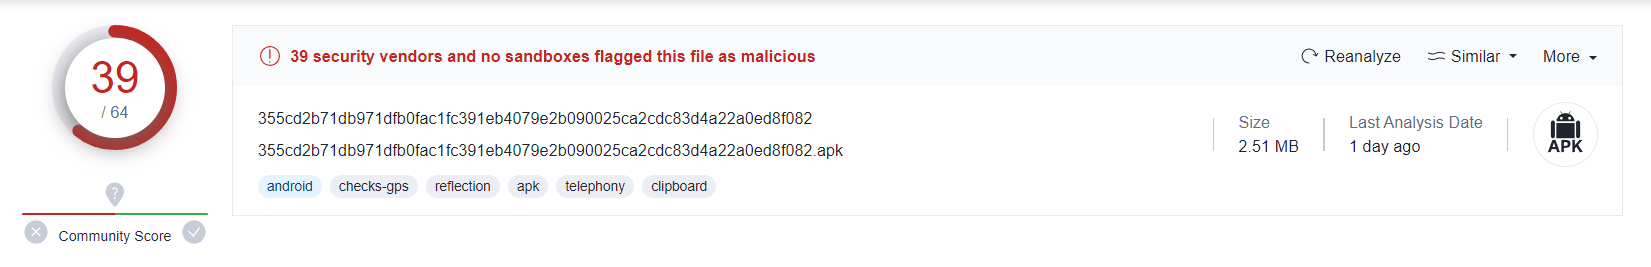
\includegraphics[width=1\textwidth]{./images/screenshot/SanaSystem/ReviewSanaSystem.png}
    \caption{Review score of Sana System}
    \label{fig:SanaReview}
\end{figure}

As it can be seen the score of 39 out of 64 indicate a very high chance of being a virus. In general many anti-malwares, like Avast or Kaspersky, flag this software as malicious as it can be seen in Fig. \ref{fig:SanaDetection}.

\begin{figure}[h!]
\centering
    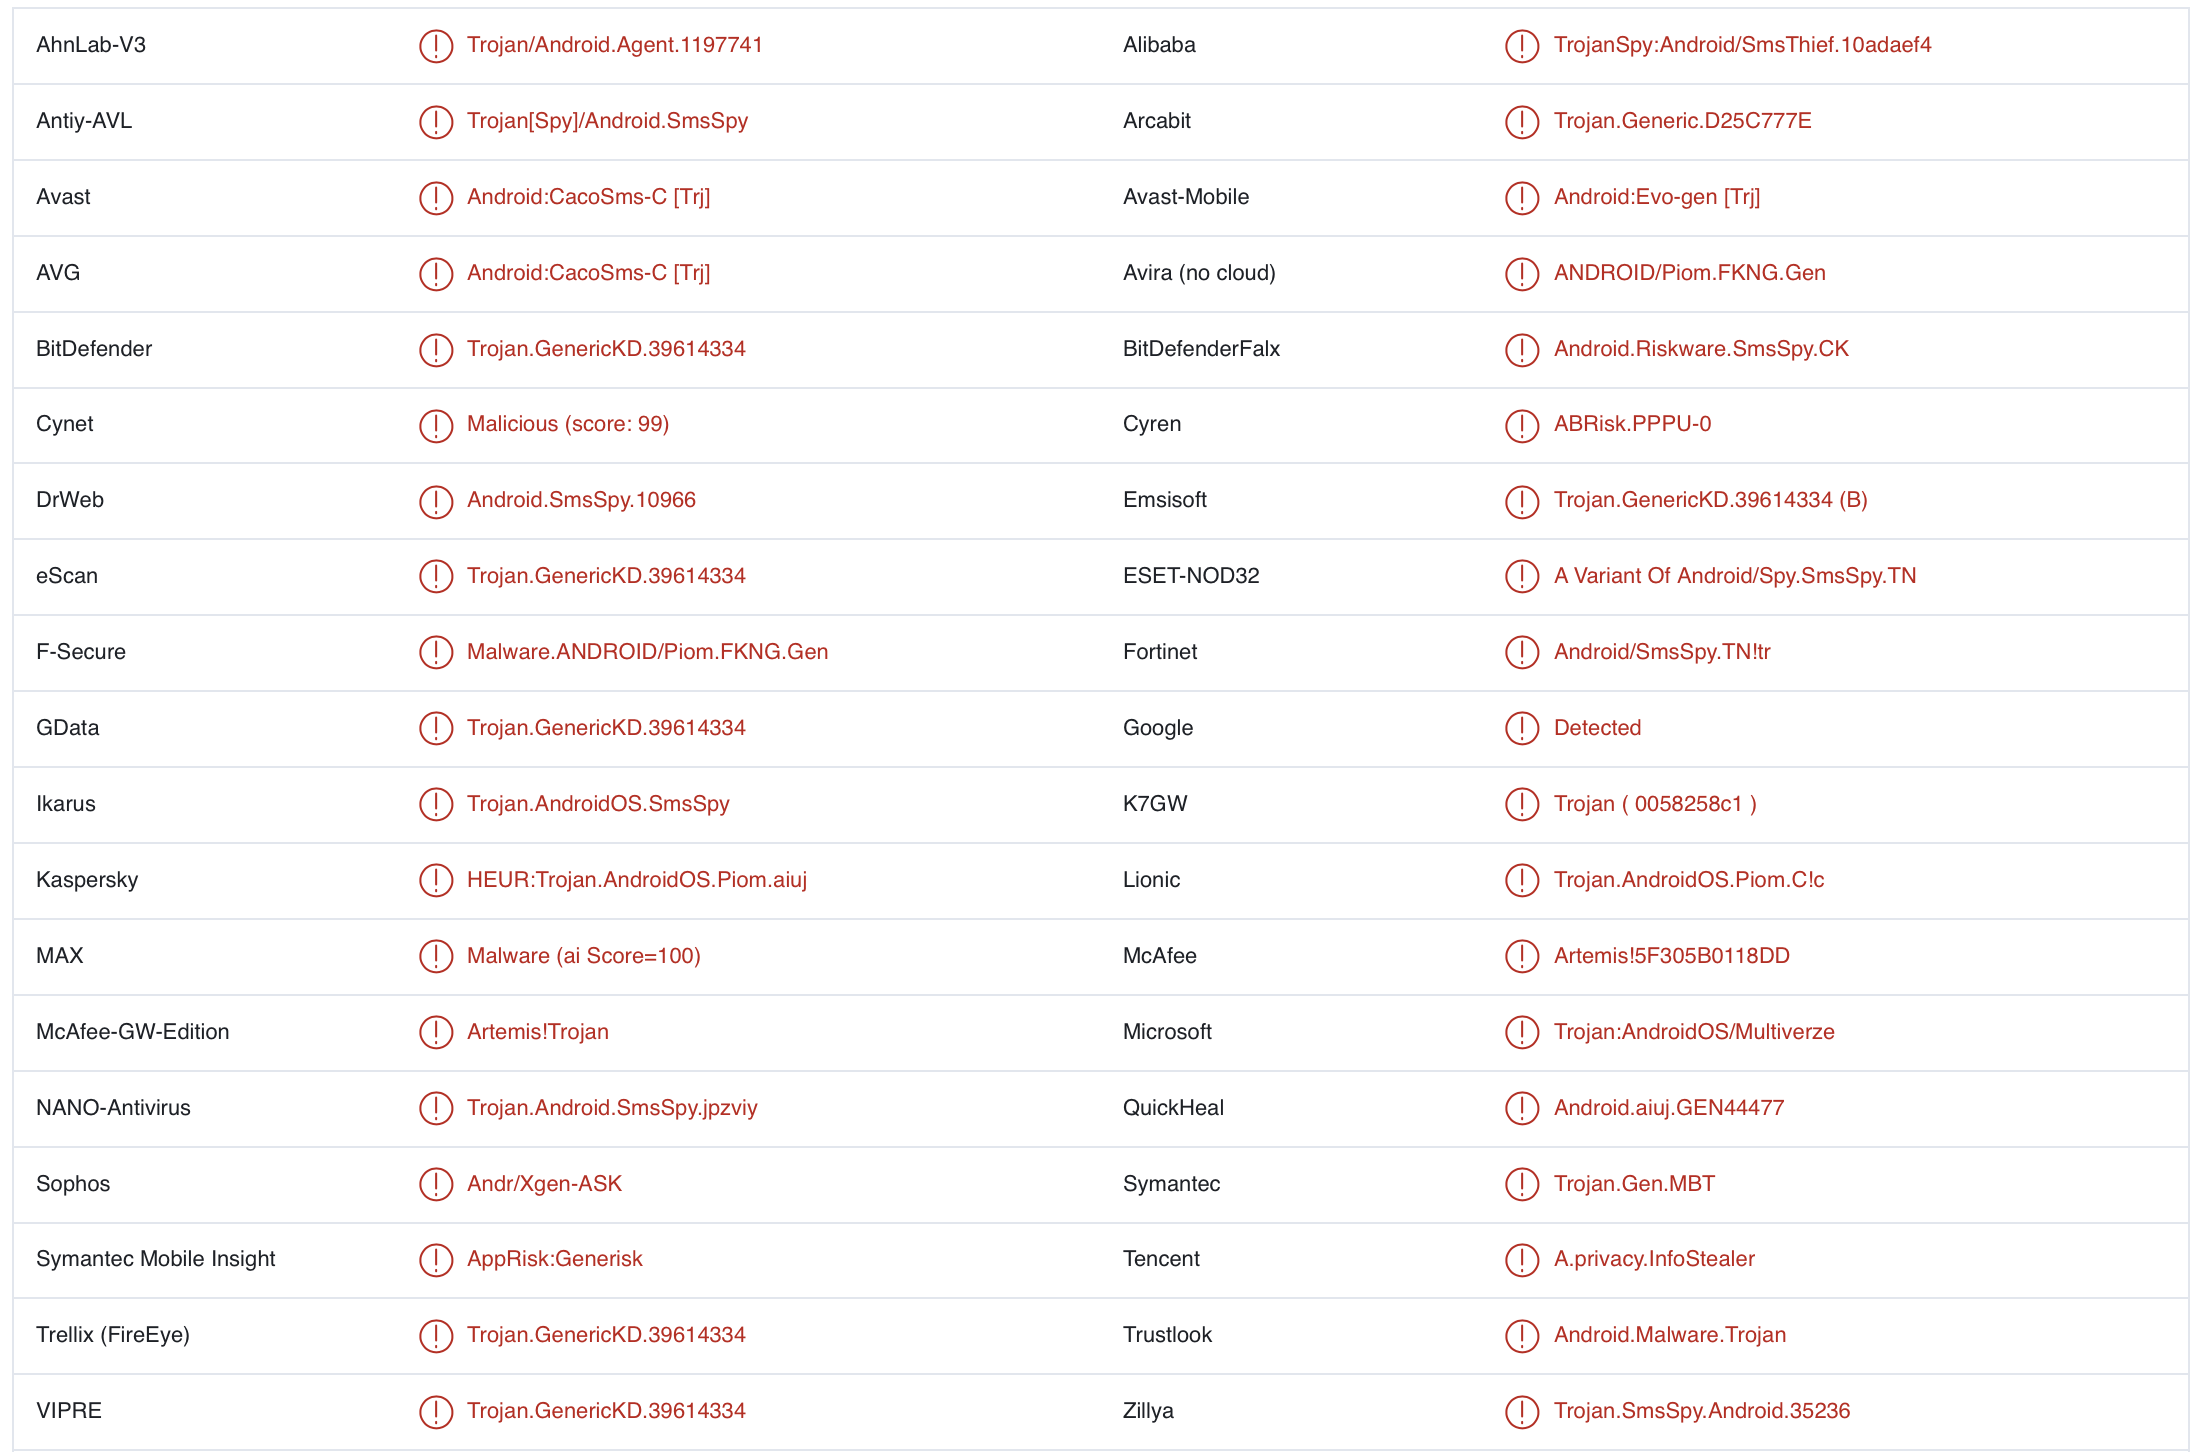
\includegraphics[width=1\textwidth]{./images/screenshot/SanaSystem/Detection.png}
    \caption{Anti-malware detection}
    \label{fig:SanaDetection}
\end{figure}

\section{MobSF}


\begin{figure}[h!]
\centering
    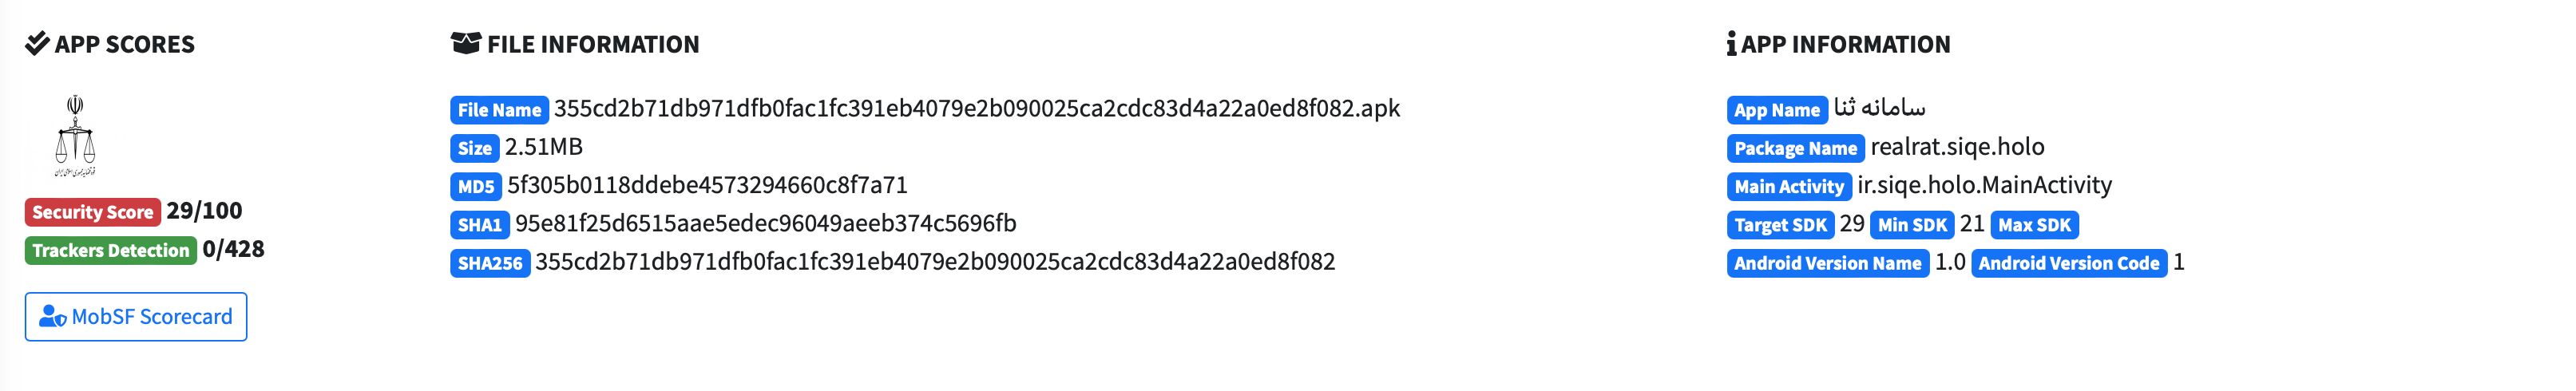
\includegraphics[width=1\textwidth]{./images/screenshot/SanaSystem/HeaderMobSF.png}
    \caption{Header of MobSF}
    \label{fig:mobsfHeader}
\end{figure}




